\documentclass[11pt,a4paper]{article}
\usepackage[T1]{fontenc}
\usepackage[utf8]{inputenc}
\usepackage{mathptmx}
\usepackage[margin=2.3cm]{geometry}
\usepackage{amsmath,amssymb,amsthm,mathtools,bm}
\usepackage{booktabs,multirow,array}
\usepackage{microtype}
\usepackage{xcolor}
\usepackage{graphicx}
\usepackage{caption}
\usepackage{float}
\usepackage{pgfplots}
\usepgfplotslibrary{groupplots}
\pgfplotsset{compat=1.17}
\usetikzlibrary{arrows.meta,positioning}
\usepackage[colorlinks=true,linkcolor=navy,citecolor=navy,urlcolor=navy]{hyperref}
\usepackage[capitalise,noabbrev]{cleveref}

\definecolor{navy}{HTML}{1E2761}
\definecolor{sA}{HTML}{2A78D6}
\definecolor{sB}{HTML}{EB6834}
\definecolor{sC}{HTML}{1BAF7A}
\definecolor{sD}{HTML}{EDA100}
\definecolor{ink}{HTML}{4B5563}
\captionsetup{font=small,labelfont=bf}
\pgfplotsset{every axis/.append style={tick label style={font=\scriptsize,color=ink},label style={font=\small,color=ink},title style={font=\small},axis line style={ink!60},tick style={ink!60},grid style={gray!20}}}

\theoremstyle{plain}
\newtheorem{theorem}{Theorem}
\newtheorem{proposition}[theorem]{Proposition}
\newtheorem{lemma}[theorem]{Lemma}
\newtheorem{corollary}[theorem]{Corollary}
\theoremstyle{definition}
\newtheorem{definition}{Definition}
\newcommand{\repourl}{\url{https://github.com/MDP2004/MuST-Walk}}
\newcommand{\R}{\mathbb{R}}
\newcommand{\E}{\mathbb{E}}
\newcommand{\Var}{\operatorname{Var}}
\newcommand{\Cov}{\operatorname{Cov}}
\newcommand{\tH}{\widetilde{H}}
\DeclareMathOperator{\AP}{AP}

\title{\textbf{MuST-Walk: Multi-Scale Temporal Walk Encodings for Efficient Temporal Link Prediction}\\[4pt]
\large DAL 518: Graph Machine Learning, Project 4.3}
\author{Abhi Raj (23125003) \and Manas Dnyaneshvar Patil (23125020) \and Kamranjeet Singh (23125016)}
\date{November 2026\\[3pt]\normalsize Code and results: \repourl}

\begin{document}
\maketitle

\begin{abstract}
Temporal link prediction asks which pair of nodes will interact next in a stream of timed edges. TPNet encodes temporal walks efficiently with a random-projection sketch, but it gives each dataset one exponential decay rate, and so one memory length. We ask whether several rates on one shared projection do better, at what cost, and on which graphs. We propose two methods: MuST-Walk keeps $J$ sketches over one projection and fuses them, and MuST-HN adds training on historical negatives. We prove the walk recursion and the sketch identity from first principles, extend the projection guarantee to $J$ scales, derive the exact noise of each pair feature, and give a lazy update that removes the batch-wide write from the per-edge cost. Inspecting the pipeline, we remove a same-timestamp leak and show that on yearly data the sketch reads a one-step-old edge at full weight. We evaluate on six DyGLib and four TGB datasets against TPNet. MuST-Walk passes our per-dataset rule on 3 of 6 DyGLib datasets but wins 9 of 18 seeds, and its cross-dataset test is not supported. MuST-HN beats TPNet by $+9.01$ to $+26.48$ AP on all six datasets, 18 of 18 seeds, though that gain comes from the training change and not from multi-scale, and it costs random-negative AP on 4 of 6 datasets. To explain these results we measure each graph's structure and test each decay rate with no neural model. Most of the multi-scale gain has one cause. A pair never seen in its stored direction cannot be a historical negative, so it must be real. Fast decay reads such a pair and a long-idle pair as the same zero, and slower scales separate them. With those pairs removed, the feature-level ladder gain falls from $+13.65$ to $+1.32$ AP on US Legis.\ and from $+27.77$ to $+5.18$ on Can. Parl. A no-learning rule that uses this fact beats both proposed methods on four of six datasets. On near-complete graphs walks saturate, and the sketch is blind to edge direction, which explains the failures there.
\end{abstract}

\section{Problem statement}\label{sec:intro}
A continuous-time dynamic graph is a stream of timestamped edges. Given all edges before time $t$, temporal link prediction scores whether nodes $u$ and $v$ interact at $t$. The task underlies recommendation, communication analysis and forecasting of relations between institutions. Two signals dominate it: pairs that interacted recently tend to interact again, and pairs connected through shared neighbours tend to interact next.

This project studies scalable, time-aware structural encodings based on temporal walks rather than static paths. Walk encodings can capture how nodes are connected through time, but counting walks exactly costs too much on a stream. The goal is to keep the efficiency of a sketch while capturing reachability over long time ranges, and to understand when doing so helps.

\subsection{Formulation}\label{sec:problem}
Let $\mathcal{G}=\{(u_i,v_i,t_i)\}_{i=1}^{E}$ with $t_1\le t_2\le\dots$, on $n$ nodes. Pairs are stored in an order $(u,v)$, and we call that the stored direction. The model outputs a score for a query $(u,v,t)$ using only edges strictly before $t$. Data is split in time order, 70/15/15. We report average precision,
\begin{equation}\label{eq:ap}
\AP=\sum_{i}(R_i-R_{i-1})\,P_i,
\end{equation}
over distinct score thresholds with recall $R_i$ and precision $P_i$, so tied scores form one step. Positives are real test edges. A test needs negatives, and the choice defines the task.
\begin{definition}[Negative types]
A \emph{random} negative pairs a query source with a random destination. A \emph{historical} negative \cite{poursafaei} is a stored pair $(u,v)$ seen strictly before the batch and not active in the batch's time interval. An \emph{inductive} negative involves unseen nodes. We use historical AP as the primary metric.
\end{definition}

\subsection{Research questions and findings}
\begin{itemize}\itemsep1pt
\item \textbf{RQ1. Do several decay rates on one projection beat one?} Not in general. MuST-Walk passes a per-dataset rule on 3 of 6 datasets, and it wins 9 of 18 seeds (\cref{sec:results}).
\item \textbf{RQ2. On which graphs, and why?} Where fast decay ties never-seen pairs with long-idle pairs, on graphs with turnover and many new pairs. Most of that gain comes from how the historical test is built (\cref{sec:why}).
\item \textbf{RQ3. What does it cost?} Time and memory linear in $J$, with no new approximation in the sketch, and a lazy update that removes the batch-wide write (\cref{sec:maintain}).
\item \textbf{RQ4. What do these benchmarks measure?} Random AP is capped near a computable level on near-complete graphs, and historical AP gives a share of positives away (\cref{sec:eval}).
\end{itemize}
Our contributions are two methods, MuST-Walk and MuST-HN, a self-contained treatment of the walk sketch with exact noise formulas, the lazy update, a corrected pipeline, and a structural explanation of each outcome that we test directly. We compare each method with the TPNet baseline only; other configurations we ran are outside the scope of this paper. We do not claim historical-negative training or the leak fix as new; both have prior work, cited where used.

\section{Literature review}\label{sec:lit}
\subsection{Approaches to temporal link prediction}
Work on temporal link prediction falls into a few families. Memory-based models such as TGN \cite{tgn} keep a state per node, updated by events. Walk-sampling models such as CAWN \cite{cawn} sample anonymous walks around each pair. Sequence models such as DyGFormer \cite{dygformer} encode co-occurrence in first-hop histories. Encodings built on a whole supra-graph, such as SLATE \cite{slate}, apply a Laplacian encoding to a multi-layer graph. TPNet \cite{tpnet} shows that many relative encodings are choices of a walk score and a readout, and it maintains the walk matrix through a random projection. TPNet is our baseline, and the next two subsections review it.

Three further lines of work shape this project. On evaluation, Poursafaei et al.\ \cite{poursafaei} introduced historical and inductive negatives, and TGB \cite{tgb} provides standard benchmarks. On training, ENS \cite{ens}, CurNM \cite{curnm} and ATNSF \cite{atnsf} use harder negatives. On batching, Zhang et al.\ \cite{snam} and Lampert et al.\ \cite{lampert} study how same-time information reaches batched models. Forward decay \cite{forward} supplies the idea behind the update rule.

\subsection{TPNet: temporal walk matrices}
\begin{definition}[Temporal walk and score]
A $k$-step temporal walk from $w_0$ is $W=[(w_0,t_0),\dots,(w_k,t_k)]$ with $t_0>t_1>\dots>t_k$, where each $(w_{i-1},w_i)$ interacted at time $t_i$, in either stored direction. Its score at time $t\ge t_1$ is
\begin{equation}\label{eq:score}
s_t(W)=\prod_{i=1}^{k} e^{-\lambda(t-t_i)},\qquad \lambda\ge 0.
\end{equation}
The walk matrix $A^{(l)}(t)\in\R^{n\times n}$ has entries $A^{(l)}_{u,w}(t)=\sum_{W}s_t(W)$ over $l$-step walks from $u$ to $w$ using edges up to time $t$, and $A^{(0)}=I$.
\end{definition}
A walk leaves its start over its newest edge and moves to strictly older edges. Two lemmas give the whole dynamics of $A$.
\begin{lemma}[Aging]\label[lemma]{lem:age}
With no event in $(t,t']$, $A^{(l)}(t')=e^{-\lambda l(t'-t)}A^{(l)}(t)$.
\end{lemma}
\begin{proof}
The walk set is unchanged, and each of the $l$ factors in \eqref{eq:score} gains $e^{-\lambda(t'-t)}$.
\end{proof}
\begin{lemma}[Event recursion]\label[lemma]{lem:event}
Let edge $(u,v,t)$ have a timestamp strictly above all earlier edges. Then for $l\ge1$,
\begin{equation}\label{eq:event}
A^{(l)}_{u,\cdot}(t^{+})=A^{(l)}_{u,\cdot}(t)+A^{(l-1)}_{v,\cdot}(t),\qquad A^{(l)}_{v,\cdot}(t^{+})=A^{(l)}_{v,\cdot}(t)+A^{(l-1)}_{u,\cdot}(t),
\end{equation}
and all other rows are unchanged.
\end{lemma}
\begin{proof}
Times strictly decrease along a walk, so a walk using the new edge uses it exactly once and as its first hop. Hence new $l$-step walks from $u$ are that edge followed by an $(l-1)$-step walk from $v$ over strictly older edges, and likewise from $v$. The first hop has factor $e^{-\lambda(t-t)}=1$, and the remaining factors equal the score of the shorter walk at $t$. No other start node gains a walk.
\end{proof}

\subsection{TPNet: the sketch}\label{sec:sketch}
Let $P\in\R^{n\times d_R}$ have independent $\mathcal{N}(0,1/d_R)$ entries. TPNet stores $H^{(0)}=P$ and $H^{(l)}\in\R^{n\times d_R}$, initially zero for $l\ge1$, and on $(u,v,t)$ applies, for $l=k,\dots,1$,
\begin{equation}\label{eq:update}
H_u^{(l)}\leftarrow H_u^{(l)}+e^{\lambda t}H_v^{(l-1)},\qquad H_v^{(l)}\leftarrow H_v^{(l)}+e^{\lambda t}H_u^{(l-1)}.
\end{equation}
The descending order of $l$ makes each layer read the previous value of the layer below. The stored form carries a positive exponent although every walk weight decays. The next result resolves this.
\begin{theorem}[Sketch identity]\label{thm:sketch}
Define $\tH^{(l)}(t):=e^{-\lambda l t}H^{(l)}(t)$. If all timestamps differ, then for all $l$ and $t$,
\begin{equation}\label{eq:identity}
\tH^{(l)}(t)=A^{(l)}(t)\,P .
\end{equation}
\end{theorem}
\begin{proof}
Induct over events. At the start both sides are zero for $l\ge1$, and $\tH^{(0)}=P=A^{(0)}P$ always. Between events $H^{(l)}$ is constant, so $\tH^{(l)}(t')=e^{-\lambda l(t'-t)}\tH^{(l)}(t)$, which matches \cref{lem:age}. At event $(u,v,t)$, multiply \eqref{eq:update} by $e^{-\lambda lt}$:
\[
\tH_u^{(l)}(t^{+})=\tH_u^{(l)}(t)+e^{-\lambda lt}e^{\lambda t}H_v^{(l-1)}(t)=\tH_u^{(l)}(t)+e^{-\lambda(l-1)t}H_v^{(l-1)}(t)=\tH_u^{(l)}(t)+\tH_v^{(l-1)}(t).
\]
Using \eqref{eq:identity} before the event, this equals $\bigl(A^{(l)}_{u,\cdot}(t)+A^{(l-1)}_{v,\cdot}(t)\bigr)P$, which is the row in \eqref{eq:event} times $P$.
\end{proof}
So old edges are not shrunk when stored. New edges are inflated relative to them, and the readout divides by the current inflation. For $l=1$, $e^{-\lambda T}H_u^{(1)}(T)=\sum_i e^{-\lambda(T-t_i)}P_{v_i}$ over $u$'s contacts. This is the forward-decay construction of Cormode et al.\ \cite{forward}.

The positive form cannot run on our data. UN Vote spans 71 yearly steps, so $\lambda t\approx 2.2\times10^{4}$ at $\lambda=10^{-5}$, while a double overflows at $e^{709}$. The released code therefore stores $\tH$ and ages it, multiplying layer $l$ by $e^{-\lambda l\Delta}$ for a time step $\Delta$. \Cref{sec:maintain} deals with the cost.

\paragraph{Batches.} The code applies edges in batches. For batch $B$ with largest time $T$, it ages to $T$ and then adds $e^{-\lambda(T-s)}\tH^{(l-1)}$ for each edge at time $s$, using values from before the batch.
\begin{proposition}[Batch semantics]\label[proposition]{prop:batch}
After a sequence of batches, $\tH^{(l)}=\bar A^{(l)}P$, where $\bar A^{(l)}$ counts exactly the walks that use at most one edge from each batch, with strictly decreasing times between batches. Edges of equal time in one batch never chain, as the definition requires.
\end{proposition}
\begin{proof}
Induct over batches. Each added message reads layer $l-1$ as it stood before the batch, so a new walk has one edge from this batch as first hop followed by a walk over earlier batches. Its first factor at $T$ is $e^{-\lambda(T-s)}$, and the aged lower layer gives the remaining factors at $T$.
\end{proof}
When one yearly step forms one batch the walk matrix is exact. When a step is split across batches, edges of the same year can chain, which is wrong. When a 200-edge batch holds distinct times, walks inside the batch are lost at depth $l\ge2$, a small approximation that TPNet shares.

For nodes $u,v$ the model forms inner products among $\{r_u^{(l)},r_v^{(l)}\}_{l=0}^{k}$, with $r_u^{(l)}=\tH_u^{(l)}$, giving a pair feature of dimension $D=(2k+2)^2$. Each inner product is clamped at zero and passed through $\log(1+x)$ and an MLP. It joins neighbour and time information in an MLP-Mixer encoder and a link predictor \cite{tpnet}. 

\section{Problems with existing work}\label{sec:problems}
Each family has a limit. Node memory is compact but does not by itself describe how two nodes relate. Walk sampling captures pair relations at the price of sampling for every query. Sequence models reach only limited structural depth. Supra-graph encodings need memory close to the full multi-layer graph, which limits scale.

TPNet avoids these limits, in time that does not depend on graph size in theory, but it leaves four problems open.
\begin{enumerate}\itemsep1pt
\item \textbf{One memory length.} A single rate $\lambda$ gives every pair the same exponential memory. A real graph need not have an exponential memory, and short and long ranges share one scale.
\item \textbf{A rate tied to the time unit.} On yearly data with timestamps in seconds, $\lambda=10^{-5}$ gives $e^{-315}$ per year. What that memory actually does has not been examined.
\item \textbf{Cost in practice.} The analysis promises a per-edge cost independent of $n$, but the released code ages every row before each batch, for numerical safety.
\item \textbf{Same-time information.} Fixed-size batches split a yearly timestamp, so same-year edges reach the sketch before prediction.
\end{enumerate}
The benchmarks have problems of their own. Random negatives are often true edges, 95.7\% of them on UN Vote, and historical negatives give some positives away. \Cref{sec:why} analyses both.

\section{Our methods}\label{sec:method}
\subsection{Method 1: MuST-Walk}
Choose rates $\lambda_1,\dots,\lambda_J$ and maintain layers $H_j^{(l)}$ for each, with one shared $H_j^{(0)}=P$. Since \eqref{eq:update} runs unchanged per scale, \cref{thm:sketch} holds per scale, so the extension adds no approximation beyond the projection. Tuned rates $\lambda^\star$ come from the TPNet configuration: $10^{-5}$ on Can. Parl.\ and UN Vote, $10^{-6}$ on US Legis.\ and Enron, $10^{-7}$ on UN Trade and UCI. The ladder is $\{10\lambda^\star,\lambda^\star,\lambda^\star/10,0\}$ on UCI and Enron, and $\{10^{-5},10^{-7},2.2\times10^{-8},0\}$ on yearly data, with $10^{-6}$ added on US Legis.\ so that its tuned rate is present.

\subsection{What several rates can express}
Consider a depth-one feature that mixes scales with weights $\alpha_j$. For a pair with contacts at ages $\delta_i$,
\begin{equation}\label{eq:kernel}
\sum_j \alpha_j A^{(1)}_{\lambda_j}[u,v]=\sum_i\kappa(\delta_i),\qquad \kappa(\delta)=\sum_{j}\alpha_j e^{-\lambda_j\delta}.
\end{equation}
A single scale fixes $\kappa$ to one exponential. Several scales give a kernel in the span of exponentials, which is what a learned fusion can reach.
\begin{proposition}[Expressivity on a grid]\label[proposition]{prop:vander}
On a grid of step $\Delta$ let $x_j=e^{-\lambda_j\Delta}$. If the $x_j$ are distinct, then for any target values on $J$ consecutive ages there is a unique $\alpha$ with $\kappa$ equal to them. If two $x_j$ are numerically equal, those scales add nothing.
\end{proposition}
\begin{proof}
On ages $a\Delta$, $a=0,\dots,J-1$, the system has matrix $W_{aj}=x_j^{a}$, a Vandermonde matrix with determinant $\prod_{i<j}(x_j-x_i)$. This is nonzero exactly when the $x_j$ are distinct.
\end{proof}
\begin{corollary}[The usable window of a rate]\label[corollary]{cor:window}
On data with smallest step $\Delta$ and span $T$, a rate with $\lambda T\ll1$ behaves like $\lambda=0$, since $1-\lambda\delta\le e^{-\lambda\delta}\le1$ for all ages $\delta\le T$. A rate with $\lambda\Delta\gg1$ gives $x\approx0$. Only rates with $1/T\lesssim\lambda\lesssim1/\Delta$ are distinct.
\end{corollary}
On yearly data the MuST ladder gives $x\approx\{0,\ 0.043,\ 0.5,\ 1\}$, four usable scales. The uniform ladder $\{10^{-4},10^{-5},10^{-6},10^{-7}\}$ gives $\{0,\ 0,\ 2\times10^{-14},\ 0.043\}$, about two. Half-lives $\ln2/\lambda$ are 19.3 hours at $10^{-5}$, 8 days at $10^{-6}$, 80 days at $10^{-7}$ and one year at $2.2\times10^{-8}$.

\subsection{Exact noise of the sketch}
The pair features of \cref{sec:sketch} are sketched inner products, so we need their exact error.
\begin{proposition}[Exact noise of a sketched inner product]\label[proposition]{prop:noise}
For fixed $a,b,c,e\in\R^n$,
\begin{align}
\E\langle aP,bP\rangle&=\langle a,b\rangle,\label{eq:mean}\\
\Var\langle aP,bP\rangle&=\tfrac{1}{d_R}\bigl(\|a\|^2\|b\|^2+\langle a,b\rangle^2\bigr),\label{eq:var}\\
\Cov\bigl(\langle aP,bP\rangle,\langle cP,eP\rangle\bigr)&=\tfrac{1}{d_R}\bigl(\langle a,c\rangle\langle b,e\rangle+\langle a,e\rangle\langle b,c\rangle\bigr).\label{eq:cov}
\end{align}
\end{proposition}
\begin{proof}
Columns of $P$ are independent. In one column, $X_a=\sum_i a_iP_{ic}$ and its analogues are jointly Gaussian, zero-mean, with $\Cov(X_a,X_b)=\langle a,b\rangle/d_R$. The inner product is a sum over $d_R$ columns of $X_aX_b$, which gives \eqref{eq:mean}. By Isserlis' theorem \cite{isserlis}, $\Cov(X_aX_b,X_cX_e)=\Cov(X_a,X_c)\Cov(X_b,X_e)+\Cov(X_a,X_e)\Cov(X_b,X_c)$. Summing over columns gives \eqref{eq:cov}, and $c=a,e=b$ gives \eqref{eq:var}.
\end{proof}
\begin{corollary}[Resolution of one contact]\label[corollary]{cor:res}
Let $a=A^{(1)}_{u,\cdot}$. The feature $\langle r_u^{(1)},P_v\rangle$ estimates $a_v$ with variance $(\|a\|^2+a_v^2)/d_R$. If $u$ has $m$ contacts of equal weight, the signal-to-noise ratio for one of them is
\begin{equation}\label{eq:rho}
\rho=\sqrt{\frac{d_R}{m+1}} .
\end{equation}
\end{corollary}
\begin{proof}
Take $b=e_v$ in \eqref{eq:var}. With unit weights $a_v=1$ and $\|a\|^2=m$, so $\rho=a_v/\sqrt{\Var}=\sqrt{d_R/(m+1)}$.
\end{proof}
The code sets $d_R=\min(\lfloor\ln 2E\rfloor\cdot10,\,n)$, between 110 and 140 on our datasets. \Cref{cor:res} therefore ties the sketch to graph structure: a node with about $d_R$ contacts resolves one contact at about one standard deviation. Dense graphs sit there, as \cref{sec:data} shows.

\subsection{Why one shared projection}
Sharing $P$ saves $J-1$ copies of $n\,d_R$ numbers, and it makes comparison across scales meaningful.
\begin{proposition}[Inner products across scales]\label[proposition]{prop:cross}
Let $r_u^{(l)}(\lambda)=A_{\lambda}^{(l)}[u,:]\,P$. With one shared $P$,
\begin{equation}
\E\bigl\langle r_u^{(l)}(\lambda_a),\,r_v^{(m)}(\lambda_b)\bigr\rangle=\sum_{w}A^{(l)}_{\lambda_a}[u,w]\,A^{(m)}_{\lambda_b}[v,w],
\end{equation}
a sum over shared intermediate nodes weighting $u$'s walks at rate $\lambda_a$ and $v$'s at $\lambda_b$. With independent $P_a,P_b$ the expectation is $0$.
\end{proposition}
\begin{proof}
The first claim is \eqref{eq:mean}. For independent zero-mean projections $\E[P_aP_b^{\top}]=0$.
\end{proof}
Sharing has a price, which \eqref{eq:cov} states exactly: noise across scales is correlated, and nearly equal scales produce nearly equal features and nearly equal noise, consistent with \cref{prop:vander}.

We can now state the guarantee across scales.
\begin{theorem}[Projection guarantee for $J$ scales]\label{thm:jl}
Let $\varepsilon\in(0,\tfrac12]$ and $N=J(k+1)n$. If $d_R\ge24\,\varepsilon^{-2}\log\bigl(4^{1/3}N\bigr)$, then at any fixed time, with probability at least $1-1/N$, every pair $x,y$ among the $N$ rows of all layers and scales satisfies $|\langle xP,yP\rangle-\langle x,y\rangle|\le\varepsilon\|x\|\|y\|$.
\end{theorem}
\begin{proof}
The rows depend only on the stream, not on $P$. For a unit vector $z$, $d_R\|zP\|^2\sim\chi^2_{d_R}$, and the Chernoff bound gives
$\Pr\bigl(|\|zP\|^2-1|>\varepsilon\bigr)\le2\exp\bigl(-\tfrac{d_R}{2}(\tfrac{\varepsilon^2}{2}-\tfrac{\varepsilon^3}{3})\bigr)\le2e^{-d_R\varepsilon^2/6}$,
using $\varepsilon\le\frac12$. For unit $x,y$, polarisation gives $\langle x,y\rangle=\frac14(\|x+y\|^2-\|x-y\|^2)$, and if both norms are preserved up to factor $1\pm\varepsilon$ the error is at most $\frac{\varepsilon}{4}(\|x+y\|^2+\|x-y\|^2)=\varepsilon$. A union bound over at most $N^2$ pairs and two norms per pair gives failure probability at most $4N^2e^{-d_R\varepsilon^2/6}$. The assumption says $d_R\ge8\varepsilon^{-2}\log(4N^3)$, so this is at most $4N^2(4N^3)^{-4/3}\le1/N$.
\end{proof}
This is a Johnson--Lindenstrauss argument \cite{jl}, and TPNet states the single-scale version \cite{tpnet}. Moving from TPNet's $N=(k+1)n$ to $J(k+1)n$ adds only $\log J$. The cap $d_R\le n$ and the width in use matter more: for $\varepsilon=\frac12$ the theorem asks for $d_R\approx810$ to $1{,}040$ on our datasets, against 110 to 140 in the code. At the width in use the bound corresponds to $\varepsilon$ between 1.21 and 1.53, so the guarantee is vacuous and \cref{prop:noise} is the operative result.

\subsection{Fusion}
Let $f_j\in\R^D$ be the per-scale pair features and $f_b$ the feature at the tuned rate. Concatenation, $f=[f_1,\dots,f_J]\in\R^{JD}$, is our main configuration. It contains the tuned-rate feature, so in principle it loses nothing. Gated residual fusion is
\begin{equation}\label{eq:gate}
f=f_b+\beta\sum_{j=1}^{J}\alpha_jf_j,\qquad\alpha=\mathrm{softmax}\bigl(g_\phi([f_1,\dots,f_J])\bigr),\quad\beta_0=0,
\end{equation}
so training starts exactly at TPNet, and average fusion fixes $\alpha_j=1/J$.

\subsection{Method 2: MuST-HN}
MuST-HN is MuST-Walk with historical-negative training. We replace about half of the fake training pairs with pairs seen strictly before the batch and not active in its interval, and we select the best epoch on historical validation. Historical negatives come from \cite{poursafaei}. Training on them is not a new idea; see ENS \cite{ens}, CurNM \cite{curnm} and ATNSF \cite{atnsf}.

\subsection{Efficiency: the lazy update}\label{sec:maintain}
\Cref{eq:update} touches $2k$ vectors per edge, so $O(k\,d_R)$ per edge. Ageing must touch every row, because every row ages. For $b$ edges per batch,
\begin{equation}\label{eq:eager}
T_{\text{eager}}=O\bigl(Jk\,d_R(n+b)\bigr)\ \text{per batch}=O\bigl(Jk\,d_R(1+n/b)\bigr)\ \text{per edge},
\end{equation}
which grows with $n$.

Store $\hat H^{(l)}$ and a scalar $c_l$ with $c_0=1$, keeping the invariant $\tH^{(l)}=c_l\hat H^{(l)}$.
\begin{proposition}[Lazy update]\label[proposition]{prop:lazy}
Aging by $\Delta$ with $c_l\leftarrow c_le^{-\lambda l\Delta}$, and an event of weight $w$ with
\begin{equation}\label{eq:lazy}
\hat H_u^{(l)}\leftarrow\hat H_u^{(l)}+w\,\frac{c_{l-1}}{c_l}\,\hat H_v^{(l-1)},
\end{equation}
preserve the invariant and reproduce the decay form exactly in real arithmetic. If $c_l$ falls below $\theta=10^{-12}$ the layer is written out and $c_l$ reset to 1. With $\bar\Delta$ the mean time gap per batch, the amortised cost is
\begin{equation}\label{eq:lazycost}
T_{\text{lazy}}=O(Jk\,d_R)+O\Bigl(Jk^2\,\frac{n\,d_R}{b}\,\lambda\bar\Delta\Bigr)\ \text{per edge}.
\end{equation}
\end{proposition}
\begin{proof}
Aging: $c_l$ takes the factor of \cref{lem:age} and $\hat H$ is unchanged. Event: multiply \eqref{eq:lazy} by $c_l$ to get $\tH_u^{(l)}\leftarrow\tH_u^{(l)}+w\,\tH_v^{(l-1)}$. Write-out: $\hat H^{(l)}\leftarrow c_l\hat H^{(l)}$ and $c_l\leftarrow1$ leave the product fixed. Layer $l$ loses a factor $\lambda l\bar\Delta$ in log scale per batch, so it is written every $\ln(1/\theta)/(\lambda l\bar\Delta)$ batches at cost $O(n\,d_R)$. Dividing by $b$ edges per batch and summing over $l\le k$ and $J$ scales gives the second term, since $\sum_{l\le k}l=O(k^2)$.
\end{proof}
Without renormalisation $c_{l-1}/c_l=e^{+\lambda(t-t_0)}$, so the positive exponent of \eqref{eq:update} returns relative to a moving origin $t_0$. Only the second term in \eqref{eq:lazycost} grows with $n$, and it is small when $\lambda\bar\Delta\ll1$. Values match the eager form to about $10^{-7}$ in our tests.

\begin{table}[H]\centering\small
\begin{tabular}{lll}
\toprule
Operation & Cost & Note\\
\midrule
Update, eager & $O(Jk\,d_R(1+n/b))$ per edge & released code path\\
Update, lazy & $O(Jk\,d_R)$ per edge, plus renormalisation & ours\\
Strict buffer & $O(1)$ amortised per edge & each edge moved once\\
Pair feature & $O(J(2k+2)^2d_R)$ per query & $(2k+2)^2$ inner products per scale\\
Sketch state & $(1+Jk)\,n\,d_R$ numbers & $P$ stored once\\
Rebuild from scratch & $O(Jk\,d_R\,E)$ for $E$ edges & what streaming avoids\\
\bottomrule
\end{tabular}
\caption{Time and space. $k$ walk depth, $J$ scales, $n$ nodes, $d_R$ sketch width, $b$ batch size.}\label{tab:cost}
\end{table}

\paragraph{Measured efficiency.}
\begin{figure}[H]\centering
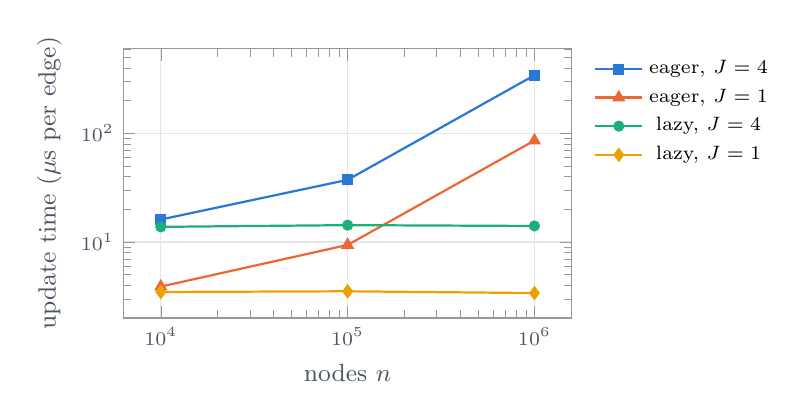
\begin{tikzpicture}
\begin{loglogaxis}[width=0.6\linewidth,height=5cm,xlabel={nodes $n$},ylabel={update time ($\mu$s per edge)},xtick={10000,100000,1000000},grid=major,legend pos=outer north east,legend style={font=\scriptsize,draw=none},ymin=2,ymax=600]
\addplot[color=sA,mark=square*,mark size=1.6pt,thick] coordinates {(10000,16.11)(100000,37.34)(1000000,342.53)};\addlegendentry{eager, $J=4$}
\addplot[color=sB,mark=triangle*,mark size=2pt,thick] coordinates {(10000,3.89)(100000,9.40)(1000000,85.84)};\addlegendentry{eager, $J=1$}
\addplot[color=sC,mark=*,mark size=1.6pt,thick] coordinates {(10000,13.79)(100000,14.30)(1000000,14.05)};\addlegendentry{lazy, $J=4$}
\addplot[color=sD,mark=diamond*,mark size=2pt,thick] coordinates {(10000,3.47)(100000,3.52)(1000000,3.39)};\addlegendentry{lazy, $J=1$}
\end{loglogaxis}
\end{tikzpicture}
\caption{Update cost on a Tesla T4, batch size 200. Gaps of about 100 s per batch mean no renormalisation occurs in the benchmark's 220 batches, so the curves show the first term of \eqref{eq:lazycost} only.}\label{fig:lazy}
\end{figure}
Eager cost grows with $n$ and lazy cost stays flat, as \eqref{eq:eager} and \eqref{eq:lazycost} predict. Lazy is 1.2, 2.6 and 24.4 times faster at $10^4$, $10^5$ and $10^6$ nodes for $J=4$. Our DyGLib datasets have at most 1,899 nodes and the largest TGB dataset has 352,637, so the 24.4 figure describes a size we benchmarked and did not train on. At $10^6$ nodes, lazy $J=4$ against $J=1$ costs 4.1 times the update time, 4.0 times the pair-feature time and 3.25 times the state. The state formula is exact: at $k=3$, $d_R=160$, $n=10^6$ it predicts 2,441.4 and 7,934.6 MiB, and we measured 2,441.5 and 7,935.1 MiB. Streaming one batch against a full rebuild at $n=10^5$ with $10^6$ past edges takes 2.47 ms against 11.93 s for $J=4$ on an RTX 6000 Ada, a factor of about 4,800.

\begin{table}[H]\centering\small
\begin{tabular}{lrrrrr}
\toprule
Minutes per run, mean of 3 seeds & US Legis. & Can. Parl. & UN Trade & UCI & Enron\\
\midrule
TPNet & 14 & 23 & 170 & 17 & 30\\
MuST-Walk & 39 & 40 & 415 & 46 & 60\\
MuST-HN & 26 & 27 & 219 & 40 & 60\\
\bottomrule
\end{tabular}
\caption{Whole-run time on Tesla T4s, including evaluation, from run logs. Early stopping changes epoch counts, so these are indicative. UN Vote is left out because its runs used mixed hardware.}\label{tab:runtime}
\end{table}
End to end, MuST-Walk took 1.7 to 2.8 times as long per run as TPNet. On tgbl-review, final evaluation took about 2.75 hours for TPNet and 5.0 for MuST-Walk on a T4.

\subsection{Correctness: the strict buffer}\label{sec:strict}
The released code updates the sketch after each 200-edge batch. One yearly timestamp holds thousands of edges across many batches, so when batch 2 of year $y$ is predicted the sketch already contains batch 1 of that year. On the four yearly datasets 96--99.9\% of test batches are affected, and these edges carry 85--99\% of the direct-connection weight. Zhang et al.\ \cite{snam} reported this first, and Lampert et al.\ \cite{lampert} describe the general batching problem. We confirmed it independently. Our fix holds incoming edges in a buffer, and before predicting a batch with earliest time $t_{\min}$ it applies exactly the waiting edges older than $t_{\min}$.
\begin{proposition}[Strict invariant]\label[proposition]{prop:strict}
With the buffer, at any query time $t$ the sketch contains an edge at time $s$ only if $s<t$, and it contains every observed edge with $s<t_{\min}$. All waiting edges of one past step are applied together, so by \cref{prop:batch} such a step never chains with itself. With no tied timestamps the buffer leaves the sketch equal to the original.
\end{proposition}
\begin{proof}
Edges enter only when $s<t_{\min}\le t$, and the rule applies all such edges. Edges of a past step are all older than the first batch lying wholly in a later step, so they enter in one application. Each edge moves once, hence $O(1)$ amortised. With distinct times, the edges of the previous batch are all older than $t_{\min}$, so the state at each prediction matches the original.
\end{proof}

\begin{table}[H]\centering\small
\begin{tabular}{lrrrr}
\toprule
TPNet, historical AP, three seeds & US Legis. & Can. Parl. & UN Trade & UN Vote\\
\midrule
Original code, 30 epochs & 91.11 & 83.43 & 71.98 & 74.94\\
Fixed code, 100 epochs & 66.25 & 81.37 & 61.00 & 57.18\\
\bottomrule
\end{tabular}
\caption{The baseline before and after correction. Code and training length both changed, so this gap is not the leak alone.}\label{tab:leak}
\end{table}
One pilot isolates the leak. On US Legis., seed 0, at 100 epochs in both arms, removing it takes TPNet from 93.41 to 67.19 and the ladder from 93.79 to 73.81. So published scores on these datasets partly reflect same-year edges.

\subsection{Correctness: what the sketch reads at query time}\label{sec:read}
\Cref{eq:score} scores a walk at the query time. The code does not: it ages the sketch only when applying edges, and a read applies no decay.
\begin{proposition}[Read weight]\label[proposition]{prop:read}
Let $\tau\le t$ be the time of the last applied edge. The model reads $A^{(l)}(\tau)P$, not $A^{(l)}(t)P$, so a direct edge at time $s$ has read weight $e^{-\lambda(\tau-s)}$. With the strict buffer on a grid of step $\Delta$, $\tau=t-\Delta$ outside batches that straddle two steps, so an edge $a\ge1$ steps old has read weight
\begin{equation}\label{eq:read}
w(a)=e^{-\lambda(a-1)\Delta}.
\end{equation}
\end{proposition}
\begin{proof}
Aging happens only inside the update, which sets the clock to the largest applied time, and a read returns stored layers. By \cref{prop:strict} the clock stands at $t-\Delta$ during step $t$. Substitute $s=t-a\Delta$.
\end{proof}

\begin{figure}[H]\centering
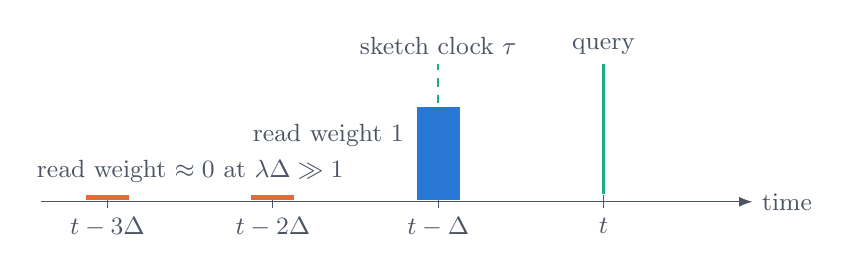
\begin{tikzpicture}[x=2.1cm,y=1cm,>=Latex]
\draw[->,ink] (-0.4,0) -- (3.9,0) node[right,font=\small]{time};
\foreach \x/\l in {0/$t-3\Delta$,1/$t-2\Delta$,2/$t-\Delta$,3/$t$} {\draw[ink] (\x,0.08) -- (\x,-0.08) node[below,font=\small]{\l};}
\fill[sB] (-0.13,0.02) rectangle (0.13,0.08);
\fill[sB] (0.87,0.02) rectangle (1.13,0.08);
\fill[sA] (1.87,0.02) rectangle (2.13,1.2);
\node[font=\small,color=ink,above] at (0.5,0.12) {read weight $\approx 0$ at $\lambda\Delta\gg1$};
\node[font=\small,color=ink,left] at (1.85,0.85) {read weight 1};
\draw[dashed,sC,thick] (2,1.25) -- (2,1.75);
\node[font=\small,color=ink,above] at (2,1.75) {sketch clock $\tau$};
\draw[sC,thick] (3,0.1) -- (3,1.75);
\node[font=\small,color=ink,above] at (3,1.75) {query};
\end{tikzpicture}
\caption{Yearly data under the strict buffer. The clock stops at the last applied step, so the previous step keeps weight 1 and decay starts from the step before it.}\label{fig:clock}
\end{figure}

\begin{table}[H]\centering\small
\begin{tabular}{lrrrrr}
\toprule
Dataset & $\lambda^\star$ & $e^{-\lambda^\star\Delta}$ & $w(1)$ & $w(2)$ & AUC\\
\midrule
US Legis. & $10^{-6}$ & $2\times10^{-14}$ & 1 & $2\times10^{-14}$ & 0.772\\
Can. Parl. & $10^{-5}$ & $10^{-137}$ & 1 & 0 in float32 & 0.966\\
UN Trade & $10^{-7}$ & 0.043 & 1 & 0.043 & 0.745\\
UN Vote & $10^{-5}$ & $10^{-137}$ & 1 & 0 in float32 & 0.610\\
\bottomrule
\end{tabular}
\caption{Yearly data, $\Delta=86400\times365$ s. Read weights measured on the real eager and lazy modules. AUC: on real data, at the first test step and the tuned rate, $\langle r_u^{(1)},r_v^{(0)}\rangle$ separating 3,000 pairs active one step ago from 3,000 seen only earlier. An erased step would give a feature near 0.}\label{tab:read}
\end{table}

So on yearly data the tuned rate does not erase the previous step. It keeps that step at full weight and drops older ones on US Legis., Can. Parl.\ and UN Vote. On UCI and Enron the clock lags by under a batch and the effect is negligible. All our results use the code as it ran, so \eqref{eq:read} is the memory these models had.

\section{Experimental setup}\label{sec:setup}
\subsection{Data and graph structure}\label{sec:data}
We use six DyGLib datasets \cite{dygformer}, opened pair by pair, and four TGB datasets \cite{tgb} evaluated without pair-level inspection of tgbl-wiki and tgbl-review. Four DyGLib graphs are yearly snapshots of institutions and two are continuous message streams.

\begin{table}[H]\centering\small\setlength{\tabcolsep}{3.6pt}
\begin{tabular}{lrrrrrrrrrr}
\toprule
Dataset & Nodes & Edges & Steps & Density & Snapshot & Degree & Gini & Transitivity & Edges/pair & $d_R$\\
\midrule
US Legis. & 225 & 60,396 & 12 & 0.661 & 0.200 & 148.2 & 0.15 & 0.81 & 3.6 & 110\\
Can. Parl. & 734 & 74,478 & 14 & 0.170 & 0.019 & 123.9 & 0.45 & 0.44 & 1.6 & 110\\
UN Trade & 255 & 507,497 & 32 & 0.639 & 0.307 & 161.5 & 0.22 & 0.82 & 24.5 & 130\\
UN Vote & 201 & 1,035,742 & 72 & 0.981 & 0.552 & 196.2 & 0.01 & 0.99 & 52.5 & 140\\
UCI & 1,899 & 59,835 & 58,911 & 0.008 & 0.0004 & 14.6 & 0.65 & 0.06 & 4.3 & 110\\
Enron & 184 & 125,235 & 22,632 & 0.132 & 0.005 & 22.8 & 0.35 & 0.37 & 56.5 & 120\\
\bottomrule
\end{tabular}
\caption{Static structure. Density: share of node pairs that ever interact. Snapshot: mean share active in one step, or one week on UCI and Enron. Degree: mean distinct partners. Gini: inequality of degree.}\label{tab:static}
\end{table}

\begin{table}[H]\centering\small\setlength{\tabcolsep}{4pt}
\begin{tabular}{lrrrrrrr}
\toprule
Dataset & Persistence & Node stay & New-node edges & Never seen & Free positives & Contacts & Separation $\rho$\\
\midrule
US Legis. & 0.786 & 0.886 & 22.7\% & 23.1\% & 34.3\% & 99.0 & 1.06\\
Can. Parl. & 0.297 & 0.920 & 1.8\% & 45.4\% & 51.3\% & 10.0 & 2.29\\
UN Trade & 0.884 & 0.986 & 0.0\% & 1.0\% & 2.0\% & 90.4 & 0.92\\
UN Vote & 0.991 & 0.996 & 0.0\% & 0.0\% & 0.3\% & 171.5 & 0.81\\
UCI & 0.209 & 0.493 & 22.9\% & 35.1\% & 42.1\% & 3.7 & 2.34\\
Enron & 0.468 & 0.809 & 1.5\% & 9.5\% & 11.2\% & 2.1 & 2.83\\
\bottomrule
\end{tabular}
\caption{Temporal structure, on test edges where it applies. Persistence: chance that a pair active in one period is active in the next (step, or week on UCI and Enron). Node stay: chance a node stays active into the next period (step, or 30 days). Never seen: positives with no contact in either direction before their batch, which is what the sketch and the test can know; counted edge by edge, the UCI figure would be lower because pairs repeat inside a batch. Free positives: never seen in stored direction (\cref{prop:free}). Contacts: median effective contacts $\|a\|_1^2/\|a\|_2^2$ at the tuned rate. Separation: median $a_v\sqrt{d_R}/\|a\|$ for test positives.}\label{tab:temporal}
\end{table}

\Cref{tab:temporal} confirms \cref{cor:res}. On the dense graphs effective contacts match or exceed $d_R$ and one contact sits near one standard deviation of noise; on the sparse graphs it sits at 2.3 to 2.8. Common-neighbour features saturate the same way. On UN Vote and UN Trade every test pair, real or fake, has a common neighbour, while the median count on UN Vote is 197 of 200 for both classes.

\paragraph{The memory of each graph.} \Cref{fig:kernel} shows the empirical memory kernel: the chance that a pair is active given the age of its last contact. This is the curve a decay kernel tries to match. Three shapes appear. US Legis.\ has a cliff: 0.77 at one step, 0.015 at two, and zero from three on, consistent with cohorts of legislators changing. UN Trade and UN Vote have long tails, since the same countries stay related for decades. Can. Parl.\ is low and flat after one step. On the streams, return probability falls smoothly from under a day to months, and much faster on UCI than on Enron. UCI pairs return after a median 20 minutes, with a 90th percentile of 2.5 days, against 22.5 hours and 21 days on Enron.

\begin{figure}[H]\centering
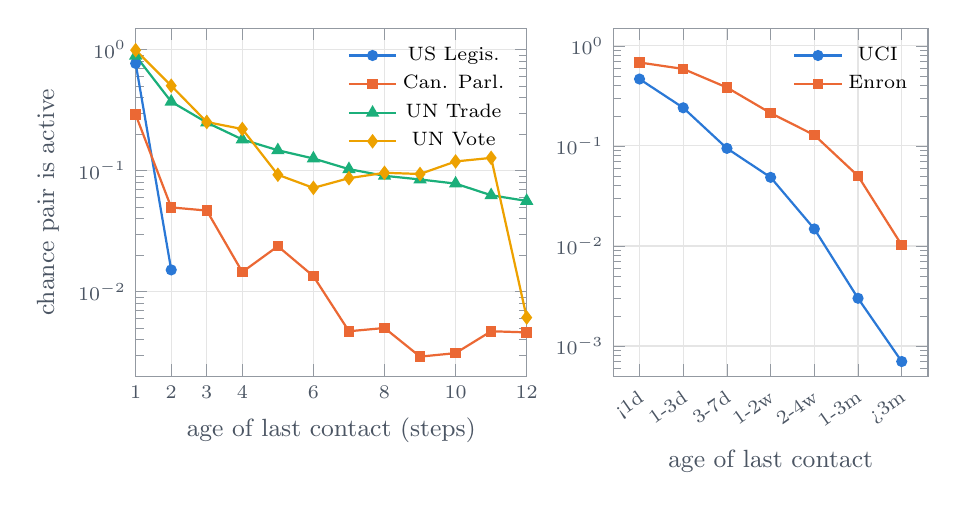
\begin{tikzpicture}
\begin{semilogyaxis}[name=a,width=0.54\linewidth,height=6cm,xlabel={age of last contact (steps)},ylabel={chance pair is active},xmin=1,xmax=12,xtick={1,2,3,4,6,8,10,12},ymin=0.002,ymax=1.5,grid=major,legend style={font=\scriptsize,draw=none,at={(0.98,0.98)},anchor=north east,fill=none}]
\addplot[color=sA,mark=*,mark size=1.6pt,thick] coordinates {(1,0.7681)(2,0.0151)};\addlegendentry{US Legis.}
\addplot[color=sB,mark=square*,mark size=1.5pt,thick] coordinates {(1,0.2894)(2,0.0496)(3,0.0467)(4,0.0145)(5,0.0237)(6,0.0134)(7,0.0047)(8,0.005)(9,0.0029)(10,0.0031)(11,0.0047)(12,0.0046)};\addlegendentry{Can. Parl.}
\addplot[color=sC,mark=triangle*,mark size=2pt,thick] coordinates {(1,0.8892)(2,0.3708)(3,0.2493)(4,0.1808)(5,0.1471)(6,0.1258)(7,0.1027)(8,0.0905)(9,0.0844)(10,0.078)(11,0.0625)(12,0.0561)};\addlegendentry{UN Trade}
\addplot[color=sD,mark=diamond*,mark size=2pt,thick] coordinates {(1,0.9885)(2,0.5026)(3,0.2517)(4,0.2203)(5,0.0923)(6,0.0719)(7,0.0865)(8,0.0958)(9,0.0937)(10,0.1189)(11,0.1273)(12,0.0061)};\addlegendentry{UN Vote}
\end{semilogyaxis}
\begin{semilogyaxis}[at={(a.east)},anchor=west,xshift=1.1cm,width=0.46\linewidth,height=6cm,xlabel={age of last contact},symbolic x coords={<1d,1-3d,3-7d,1-2w,2-4w,1-3m,>3m},xtick=data,x tick label style={rotate=35,anchor=north east},ymin=0.0005,ymax=1.5,grid=major,legend style={font=\scriptsize,draw=none,at={(0.98,0.98)},anchor=north east,fill=none}]
\addplot[color=sA,mark=*,mark size=1.6pt,thick] coordinates {(<1d,0.4658)(1-3d,0.2404)(3-7d,0.0945)(1-2w,0.0485)(2-4w,0.0148)(1-3m,0.003)(>3m,0.0007)};\addlegendentry{UCI}
\addplot[color=sB,mark=square*,mark size=1.5pt,thick] coordinates {(<1d,0.6816)(1-3d,0.588)(3-7d,0.3835)(1-2w,0.2128)(2-4w,0.1283)(1-3m,0.0501)(>3m,0.0102)};\addlegendentry{Enron}
\end{semilogyaxis}
\end{tikzpicture}
\caption{Empirical memory kernel, log scale. Left: chance of being active at a step, from 30\% of the way through the data. Right: chance of contact within the next week, weekly anchors. US Legis.\ stops at age 2 because the chance is exactly 0 from age 3.}\label{fig:kernel}
\end{figure}

Raw edge features are unscaled, with a maximum of 52,504,548 on UN Trade. 18.0--31.8\% of pre-validation edges touch held-out nodes and never enter the sketch during training, on all six datasets.

\subsection{Protocol}
\paragraph{Training.} Strict time and lazy updates, 100 epochs, patience 20, seeds 0--2, chronological 70/15/15 split. Test types are random, historical (primary) and inductive.
\paragraph{Model selection.} We keep the epoch with the best validation score and test it once; the test metrics printed each epoch were ignored. TPNet and MuST-Walk select on random validation, and MuST-HN on historical validation.
\paragraph{TGB.} MRR with the official evaluator on tgbl-wiki (999 negatives), tgbl-review (100), tgbl-uci and tgbl-enron; 30 epochs, patience 5; per-epoch validation on the first 20\% of validation edges in time order, then full validation and test. This is not the authors' protocol, so these are not leaderboard entries. As a sanity check, TPNet on tgbl-wiki gave 0.8239, within the pre-registered 0.02 of its published 0.827.
\paragraph{Decision rule.} Rules were written before results. Per dataset, a comparison passes if the mean gain is at least $+1.0$ AP and at least 2 of 3 seeds win (TGB: $+0.005$ MRR). Across datasets we planned an exact one-sided Wilcoxon test \cite{wilcoxon} with Holm correction \cite{holm} over the four comparisons of the wider experiment.
\paragraph{A flaw in that test.} With $n$ paired datasets the smallest one-sided $p$ is $2^{-n}$, so with six datasets and four tests the smallest adjusted $p$ is $4\cdot2^{-6}=0.0625>0.05$. No comparison could pass. We noticed this after the runs and did not change the rule.
\paragraph{Feature-level analysis.} To test mechanisms without a neural model, we stream exact walk matrices with the strict read, form five walk features per rate (direct contact, two-hop walks, common neighbours and each node's activity), and fit logistic regression on the validation period to predict the test period, on five negative samples. Separately we push the same features through a real projection of width $d_R$. This uses all edges before validation, so it is idealised, and it is linear. It is exploratory and was added after the main analysis.

\section{Results}\label{sec:results}
\subsection{Main comparison}
\begin{table}[H]\centering\small\setlength{\tabcolsep}{4pt}
\begin{tabular}{lrrrrrrr}
\toprule
 & & \multicolumn{3}{c}{MuST-Walk} & \multicolumn{3}{c}{MuST-HN}\\
Dataset & TPNet & AP & Gain & Seeds & AP & Gain & Seeds\\
\midrule
US Legis. & 66.25$\pm$10.86 & 75.90$\pm$4.28 & \textbf{+9.64} & 2/3 & 90.54$\pm$0.57 & \textbf{+24.28} & 3/3\\
Can. Parl. & 81.37$\pm$4.39 & 86.11$\pm$3.87 & \textbf{+4.74} & 3/3 & 91.32$\pm$0.40 & \textbf{+9.95} & 3/3\\
UN Trade & 61.00$\pm$1.20 & 60.21$\pm$0.97 & $-0.79$ & 2/3 & 87.48$\pm$0.11 & \textbf{+26.48} & 3/3\\
UN Vote & 57.18$\pm$4.22 & 59.89$\pm$0.91 & \textbf{+2.72} & 2/3 & 71.95$\pm$1.00 & \textbf{+14.77} & 3/3\\
UCI & 86.57$\pm$0.61 & 85.55$\pm$0.18 & $-1.02$ & 0/3 & 96.31$\pm$0.26 & \textbf{+9.74} & 3/3\\
Enron & 81.51$\pm$1.26 & 79.16$\pm$0.78 & $-2.35$ & 0/3 & 90.52$\pm$0.05 & \textbf{+9.01} & 3/3\\
\bottomrule
\end{tabular}
\caption{Historical test AP, mean $\pm$ std over three seeds, with gain over TPNet and seeds won against it. Bold marks a pass under the per-dataset rule. UN Vote MuST-Walk seeds 1, 2 and MuST-HN seeds 1, 2 hit time limits at 52 and 28 epochs and were tested at their best checkpoint.}\label{tab:main}
\end{table}

MuST-Walk passes on 3 of 6 datasets and wins 9 of 18 seeds. Its pre-registered cross-dataset test gives adjusted $p=0.4688$, so it is not supported. MuST-HN against TPNet was not a pre-registered comparison, so we report it as exploratory: it passes on 6 of 6 datasets and wins 18 of 18 seeds. Its gain comes from the training change, not from multi-scale: a single-rate model given the same training and selection scores about the same ($-0.25$ AP for MuST-HN, which wins 7 of 18 seeds). The gain over TPNet should therefore not be read as a gain from several decay rates.

\begin{figure}[H]\centering
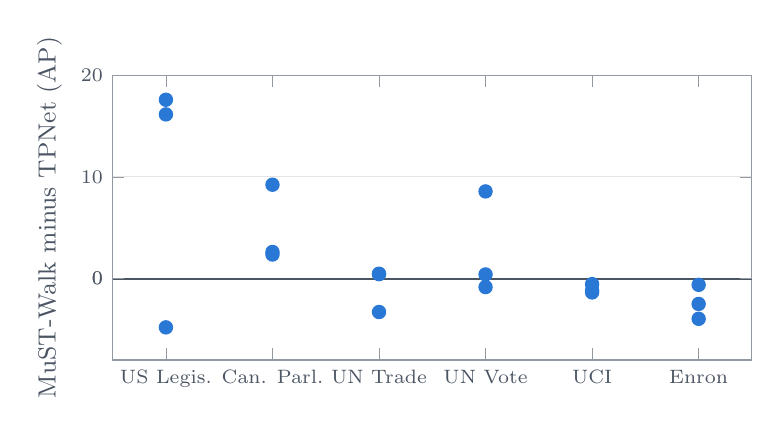
\begin{tikzpicture}
\begin{axis}[width=0.8\linewidth,height=5.2cm,symbolic x coords={US Legis.,Can. Parl.,UN Trade,UN Vote,UCI,Enron},xtick=data,ylabel={MuST-Walk minus TPNet (AP)},ymin=-8,ymax=20,ymajorgrids,enlarge x limits=0.1,extra y ticks={0},extra y tick style={grid=major,grid style={ink,thick}}]
\addplot[only marks,mark=*,mark size=2.4pt,color=sA] coordinates {(US Legis.,16.14)(US Legis.,17.58)(US Legis.,-4.79)(Can. Parl.,9.23)(Can. Parl.,2.62)(Can. Parl.,2.37)(UN Trade,0.48)(UN Trade,-3.28)(UN Trade,0.44)(UN Vote,-0.83)(UN Vote,0.41)(UN Vote,8.57)(UCI,-0.54)(UCI,-1.36)(UCI,-1.15)(Enron,-0.61)(Enron,-3.95)(Enron,-2.49)};
\end{axis}
\end{tikzpicture}
\caption{Each dot is one seed. The spread on US Legis.\ and UN Vote shows why three seeds cannot settle those means: one seed carries the UN Vote gain, and US Legis.\ runs from $-4.79$ to $+17.58$.}\label{fig:seeds}
\end{figure}

\Cref{fig:seeds} shows why the pass count needs care. Modelling each arm as normal with its observed seed spread and no true difference, the rule passes with probability 0.39, 0.35, 0.13, 0.32, 0.00 and 0.12 across the six datasets. Noise alone would pass about 1.3 datasets, and 3 or more about 11\% of the time. This is rough, since three seeds estimate a spread poorly. Random validation adds to the spread: two UN Vote TPNet seeds had validation 56.57 and scored 60.25 and 52.37, and on Can. Parl.\ later selected epochs score worse (rank correlation $-0.60$ over 6 runs).

\begin{table}[H]\centering\small
\begin{tabular}{lrrrrrr}
\toprule
AP gain over TPNet & US Legis. & Can. Parl. & UN Trade & UN Vote & UCI & Enron\\
\midrule
MuST-Walk, random & $-0.63$ & $-0.73$ & +0.41 & +0.53 & $-0.46$ & +0.09\\
MuST-Walk, inductive & +3.99 & +1.38 & +1.87 & +2.80 & $-1.32$ & +2.07\\
MuST-HN, random & +0.78 & $-3.54$ & $-6.15$ & +0.39 & $-4.95$ & $-1.02$\\
MuST-HN, inductive & +10.72 & +2.23 & +26.62 & +8.87 & +15.27 & +10.97\\
\bottomrule
\end{tabular}
\caption{Secondary metrics. MuST-Walk shows no gain on random tests (mean $-0.13$) and gains on 5 of 6 datasets on inductive tests (mean +1.80). MuST-HN costs random AP on 4 of 6 datasets and raises inductive AP on all six.}\label{tab:secondary}
\end{table}

\subsection{TGB datasets}
\begin{table}[H]\centering\small
\begin{tabular}{lrrrr}
\toprule
Test MRR & TPNet, no strict & TPNet & MuST-Walk & MuST-HN\\
\midrule
tgbl-wiki & 0.8251 & 0.8239$\pm$0.0034 & 0.8260$\pm$0.0029 & 0.7673$\pm$0.0076\\
tgbl-review & 0.4157 & 0.4033$\pm$0.0033 & 0.4025$\pm$0.0027 & 0.4939$\pm$0.0019\\
tgbl-enron & 0.636 & 0.5909$\pm$0.0011 & 0.5837$\pm$0.0064 & 0.5854$\pm$0.0128\\
tgbl-uci & 0.283 & 0.2620$\pm$0.0724 & 0.3868$\pm$0.0045 & 0.3192$\pm$0.0344\\
\bottomrule
\end{tabular}
\caption{Mean $\pm$ std over three seeds; no strict is seed 0 only. tgbl-review runs were cut by time limits: TPNet 6--9 epochs, MuST-Walk and MuST-HN 5--6. tgbl-wiki MuST-Walk seed 1 was rerun after a 2-epoch stop, by a rule fixed before the rerun: 0.8158, then 0.8228.}\label{tab:tgb}
\end{table}
MuST-Walk passes against TPNet on tgbl-uci only (+0.1248, 3 of 3 seeds), where TPNet seed 0 is low at 0.1784; on seeds 1 and 2 the gain is +0.0871 and +0.0753. MuST-HN against TPNet is $+0.091$ on tgbl-review and $+0.057$ on tgbl-uci, both on all seeds, and $-0.057$ on tgbl-wiki and $-0.005$ on tgbl-enron. TGB negatives are fixed in advance and are not all historical, so \cref{prop:free} need not apply there, which fits the mixed result; we did not test this directly. With four datasets this is descriptive, as pre-registered.

\subsection{Ablations}
Scale count, decay set and fusion ran on US Legis.\ on corrected code, as pre-registered, so they do not cover other graphs. We show each against TPNet at 66.25.
\begin{table}[H]\centering\small
\begin{tabular}{p{6.6cm}rrr}
\toprule
Configuration & Historical AP & Gain over TPNet & Seeds won\\
\midrule
$J=5$, concatenation (MuST-Walk) & 75.90$\pm$4.28 & +9.64 & 2 of 3\\
$J=3$ & 75.21$\pm$6.84 & +8.96 & 2 of 3\\
Uniform ladder $\{10^{-4},10^{-5},10^{-6},10^{-7}\}$ & 69.40$\pm$2.51 & +3.15 & 2 of 3\\
Log-spaced half-lives & 70.72$\pm$1.83 & +4.47 & 2 of 3\\
Average fusion & 80.88$\pm$2.20 & +14.63 & 3 of 3\\
Gate fusion & 81.72$\pm$3.29 & +15.47 & 3 of 3\\
Gate with per-scale LayerNorm & 72.59$\pm$5.22 & +6.34 & 2 of 3\\
\bottomrule
\end{tabular}
\caption{Fixed code, US Legis., three seeds. Descriptive.}\label{tab:abl}
\end{table}
The uniform ladder gains least, which fits \cref{prop:vander}: its scales collapse to about two values on yearly data and it has no slow scale, so it cannot break the tie of \cref{prop:tie}. Gate and average have the largest gains, possibly because they use $D$ rather than $JD$ inputs. The learned $\beta$ stayed small ($-0.04$ to $+0.03$), so the gate is not a strong switch. On a task built to need two time scales, MuST-Walk beat the best single rate by $+2.69$ and $+2.21$ in two seeds, which shows the mechanism can work. Before the correction, a pre-registered confirmation of the four-rate ladder on new seeds 3--4 of four yearly datasets gave $-0.57$ AP, 4 of 8 wins, $p=0.63$: not supported.

\section{Results explained}\label{sec:why}
\subsection{Random negatives on near-complete graphs}\label{sec:eval}
\begin{proposition}[Reference level for random AP]\label[proposition]{prop:ceil}
Let there be $N$ positives and $N$ negatives, of which a fraction $f$ are true edges at that time. A scorer that ranks every true edge above every non-edge and cannot rank among true edges has $\AP=1/(1+f)$.
\end{proposition}
\begin{proof}
All $N(1+f)$ true edges share the top score, so in \eqref{eq:ap} the first step has recall 1 and precision $N/(N+fN)$.
\end{proof}
\begin{table}[H]\centering\small
\begin{tabular}{lrrrrrr}
\toprule
 & US Legis. & Can. Parl. & UN Trade & UN Vote & UCI & Enron\\
\midrule
Fake pairs that are real, $f$ & 44.0\% & 8.3\% & 59.9\% & 95.7\% & 0.1\% & 5.3\%\\
$1/(1+f)$ & 69.4 & 92.3 & 62.5 & 51.1 & 99.9 & 95.0\\
TPNet, random AP & 69.71 & 80.55 & 67.53 & 55.23 & 97.33 & 93.26\\
\bottomrule
\end{tabular}
\caption{This is a reference level, not a hard limit: a model can pass it by ranking test pairs above other true pairs, by up to about 5.5 points here. On US Legis., UN Trade and UN Vote every model sits this close, so random AP says little there, and so does validation on it.}\label{tab:ceil}
\end{table}

\subsection{Historical negatives give some positives away}
A historical negative must have been seen in its stored direction. That simple fact has a large consequence.
\begin{proposition}[Free positives]\label[proposition]{prop:free}
Let $g$ be the share of test positives never seen in stored direction. Each such pair is certainly positive under the historical test. A scorer using only this fact has $\AP=(1+g)/2$ on a balanced test.
\end{proposition}
\begin{proof}
No historical negative has this property, so these $gN$ pairs score above everything, with precision 1 up to recall $g$. All other $(1-g)N$ positives tie with the $N$ negatives, so the next step reaches recall 1 at precision $\frac12$. Then \eqref{eq:ap} gives $g+(1-g)/2$.
\end{proof}
The floor is 67.1 on US Legis., 75.7 on Can. Parl., 71.0 on UCI and 55.6 on Enron, with no learning at all. This has a sign consequence. Under random negatives familiar pairs are likely real, so a model learns that history means positive. Under historical negatives every fake is familiar, so novelty means positive. All-time contact count at $\lambda=0$ has AUC 0.35 on US Legis.\ and Can. Parl., below chance.

\begin{proposition}[Fast decay ties novelty with absence]\label[proposition]{prop:tie}
On a grid with $\lambda\Delta\gg1$, by \eqref{eq:read} a pair whose last contact is $a\ge2$ steps old has direct read $A^{(1)}_{u,v}\approx0$, the same as a never-seen pair. No function of that feature can separate them. At $\lambda=0$ a seen pair has $A^{(1)}_{u,v}\ge1$ and a never-seen pair has 0, so a slow scale separates them exactly.
\end{proposition}
\begin{proof}
For the first claim, the contacts of the pair each contribute at most $e^{-\lambda(a-1)\Delta}$, summing to a value near 0. At $\lambda=0$ each contact contributes 1.
\end{proof}
\Cref{prop:tie} is what several rates add. At the tuned rate, 77.7\% of historical negatives and 24.7\% of positives on US Legis.\ read as zero, and 88.3\% and 53.3\% on Can. Parl. On UCI no negative reads as zero, because its tuned half-life is 80 days. Novelty is already visible there.

\subsection{Sketches cannot see direction}
No historical negative is active in its stored direction, but many are active in reverse: 81.0\% on UN Vote, 23.2\% on UN Trade, 12.7\% on US Legis.\ and under 2\% elsewhere.
\begin{proposition}[Direction blindness]\label[proposition]{prop:dir}
The sketch state is invariant under reversing the stored direction of any edge.
\end{proposition}
\begin{proof}
\Cref{eq:update} treats $u$ and $v$ symmetrically: the pair of updates is unchanged by swapping them.
\end{proof}
So the walk feature of a positive and of a same-time reversed negative contain the same pairs of rows, and only the neighbour encoder can use direction. On relations with no natural direction, such as co-voting, the stored order carries little meaning, yet the test depends on it.

\begin{table}[H]\centering\small
\begin{tabular}{lrrrrrr}
\toprule
Historical test AP & US Legis. & Can. Parl. & UN Trade & UN Vote & UCI & Enron\\
\midrule
Recency rule, direction-blind & 71.76 & 66.56 & 88.99 & 55.05 & 78.56 & 85.91\\
Recency rule, direction-aware & 69.96 & 67.18 & 94.58 & 96.27 & 75.07 & 86.32\\
Novelty-aware rule & 89.59 & 93.92 & 84.58 & 86.32 & 97.36 & 93.20\\
Floor $(1+g)/2$ & 67.1 & 75.7 & 51.0 & 50.1 & 71.0 & 55.6\\
\bottomrule
\end{tabular}
\caption{No-learning rules, exploratory. Recency rules use geometrically weighted recency on yearly data and last-seen time on UCI and Enron. The novelty-aware rule ranks pairs never seen in stored direction first, then by last contact in that direction, and is measured on our replication of the test, where the blind last-contact rule gives 70.78, 64.56, 73.52, 54.84, 78.48 and 85.53.}\label{tab:rules}
\end{table}

\subsection{Which decay rates carry signal}
\Cref{fig:rates} takes the neural model away and asks how much historical-test signal each rate carries in walk features alone. The picture differs by graph, and it matches the memory kernels of \cref{fig:kernel}. On US Legis.\ and Can. Parl.\ the curve rises toward slow rates and the ladder sits well above any single rate. On UN Trade it is flat: any rate works and the ladder adds nothing. On UN Vote everything is near chance. On UCI and Enron it peaks at a fast rate and falls toward no decay, as bursty contact predicts.

\begin{figure}[H]\centering
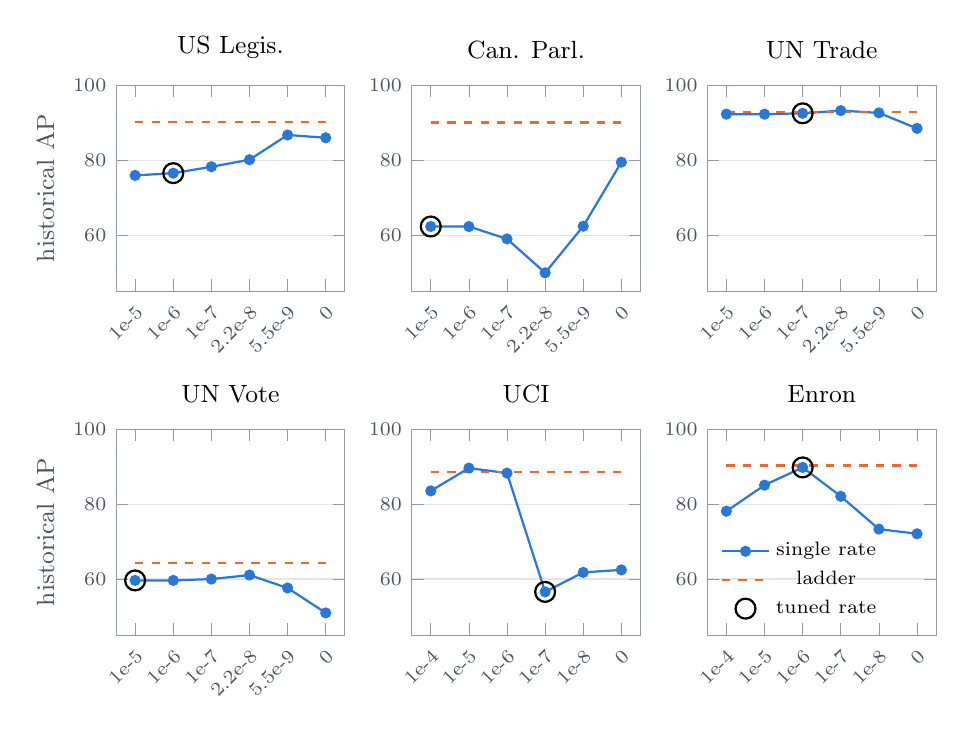
\begin{tikzpicture}
\begin{groupplot}[group style={group size=3 by 2,horizontal sep=0.85cm,vertical sep=1.75cm},width=0.37\linewidth,height=4.2cm,ymin=45,ymax=100,ymajorgrids,xtick={1,2,3,4,5,6},x tick label style={rotate=45,anchor=north east}]
\nextgroupplot[title={US Legis.},ylabel={historical AP},xticklabels={1e-5,1e-6,1e-7,2.2e-8,5.5e-9,0}]
\addplot[color=sA,mark=*,mark size=1.6pt,thick] coordinates {(1,75.91)(2,76.52)(3,78.22)(4,80.10)(5,86.70)(6,85.96)};
\addplot[color=sB,dashed,thick] coordinates {(1,90.17)(6,90.17)};
\addplot[only marks,mark=o,mark size=3.6pt,thick,color=black] coordinates {(2,76.52)};
\nextgroupplot[title={Can. Parl.},xticklabels={1e-5,1e-6,1e-7,2.2e-8,5.5e-9,0}]
\addplot[color=sA,mark=*,mark size=1.6pt,thick] coordinates {(1,62.29)(2,62.28)(3,58.98)(4,49.93)(5,62.37)(6,79.45)};
\addplot[color=sB,dashed,thick] coordinates {(1,90.06)(6,90.06)};
\addplot[only marks,mark=o,mark size=3.6pt,thick,color=black] coordinates {(1,62.29)};
\nextgroupplot[title={UN Trade},xticklabels={1e-5,1e-6,1e-7,2.2e-8,5.5e-9,0}]
\addplot[color=sA,mark=*,mark size=1.6pt,thick] coordinates {(1,92.26)(2,92.26)(3,92.48)(4,93.20)(5,92.60)(6,88.46)};
\addplot[color=sB,dashed,thick] coordinates {(1,92.92)(6,92.92)};
\addplot[only marks,mark=o,mark size=3.6pt,thick,color=black] coordinates {(3,92.48)};
\nextgroupplot[title={UN Vote},ylabel={historical AP},xticklabels={1e-5,1e-6,1e-7,2.2e-8,5.5e-9,0}]
\addplot[color=sA,mark=*,mark size=1.6pt,thick] coordinates {(1,59.63)(2,59.63)(3,59.99)(4,61.06)(5,57.61)(6,50.97)};
\addplot[color=sB,dashed,thick] coordinates {(1,64.27)(6,64.27)};
\addplot[only marks,mark=o,mark size=3.6pt,thick,color=black] coordinates {(1,59.63)};
\nextgroupplot[title={UCI},xticklabels={1e-4,1e-5,1e-6,1e-7,1e-8,0}]
\addplot[color=sA,mark=*,mark size=1.6pt,thick] coordinates {(1,83.51)(2,89.60)(3,88.26)(4,56.57)(5,61.78)(6,62.44)};
\addplot[color=sB,dashed,thick] coordinates {(1,88.66)(6,88.66)};
\addplot[only marks,mark=o,mark size=3.6pt,thick,color=black] coordinates {(4,56.57)};
\nextgroupplot[title={Enron},xticklabels={1e-4,1e-5,1e-6,1e-7,1e-8,0},legend style={font=\scriptsize,draw=none,at={(0.02,0.03)},anchor=south west,fill=none}]
\addplot[color=sA,mark=*,mark size=1.6pt,thick] coordinates {(1,78.10)(2,85.05)(3,89.78)(4,82.07)(5,73.32)(6,72.07)};\addlegendentry{single rate}
\addplot[color=sB,dashed,thick] coordinates {(1,90.31)(6,90.31)};\addlegendentry{ladder}
\addplot[only marks,mark=o,mark size=3.6pt,thick,color=black] coordinates {(3,89.78)};\addlegendentry{tuned rate}
\end{groupplot}
\end{tikzpicture}
\caption{Feature-level historical AP by decay rate, faster on the left: logistic regression on exact walk features, trained on the validation period with historical negatives, mean of five negative samples. The ring marks the tuned rate, the dashed line the ladder.}\label{fig:rates}
\end{figure}

\begin{table}[H]\centering\small\setlength{\tabcolsep}{5pt}
\begin{tabular}{lrrrrrrr}
\toprule
 & \multicolumn{3}{c}{All test positives} & \multicolumn{2}{c}{Free positives removed} & \multicolumn{2}{c}{Ladder gain}\\
Dataset & Tuned & Best single & Ladder & Tuned & Ladder & All & Removed\\
\midrule
US Legis. & 76.52 & 86.70 & 90.17 & 82.13 & 83.45 & +13.65 & +1.32\\
Can. Parl. & 62.29 & 79.45 & 90.06 & 78.83 & 84.01 & +27.77 & +5.18\\
UN Trade & 92.48 & 93.20 & 92.92 & 93.06 & 93.83 & +0.44 & +0.77\\
UN Vote & 59.63 & 61.06 & 64.27 & 61.54 & 65.16 & +4.64 & +3.62\\
UCI & 56.57 & 89.60 & 88.66 & 84.56 & 77.97 & +32.09 & $-6.59$\\
Enron & 89.78 & 89.78 & 90.31 & 92.19 & 92.27 & +0.53 & +0.08\\
\bottomrule
\end{tabular}
\caption{Feature-level test of the mechanism. Best single: rate chosen by cross-validation on the validation period. Free positives removed: positives limited to pairs seen in stored direction, so each could also have been drawn as a negative, with negatives rebalanced. Exploratory.}\label{tab:feature}
\end{table}

\begin{figure}[H]\centering
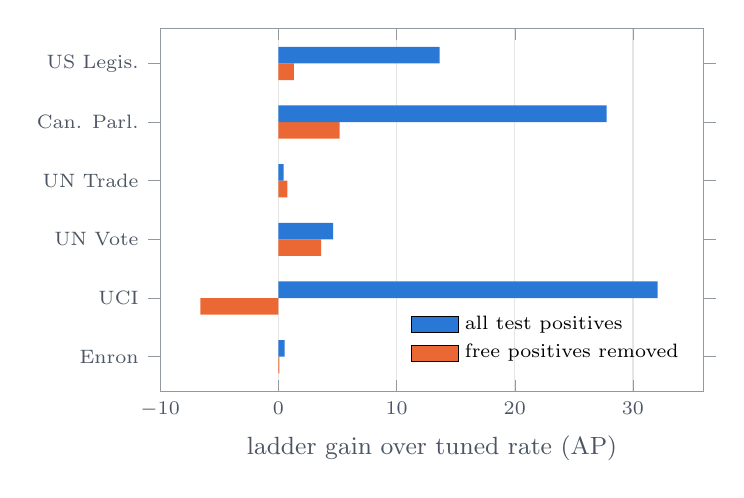
\begin{tikzpicture}
\begin{axis}[xbar=0pt,area legend,width=0.7\linewidth,height=6.2cm,symbolic y coords={Enron,UCI,UN Vote,UN Trade,Can. Parl.,US Legis.},ytick=data,y dir=normal,xlabel={ladder gain over tuned rate (AP)},xmin=-10,xmax=36,xmajorgrids,bar width=6pt,enlarge y limits=0.12,legend style={font=\scriptsize,draw=none,at={(0.98,0.05)},anchor=south east,fill=none},legend cell align=left,reverse legend]
\addplot[fill=sB,draw=none] coordinates {(0.08,Enron)(-6.59,UCI)(3.62,UN Vote)(0.77,UN Trade)(5.18,Can. Parl.)(1.32,US Legis.)};\addlegendentry{free positives removed}
\addplot[fill=sA,draw=none] coordinates {(0.53,Enron)(32.09,UCI)(4.64,UN Vote)(0.44,UN Trade)(27.77,Can. Parl.)(13.65,US Legis.)};\addlegendentry{all test positives}
\end{axis}
\end{tikzpicture}
\caption{Remove the free positives and almost all of the large ladder gains disappear, so what several rates add on these graphs is mostly the ability to spot pairs that cannot be negatives.}\label{fig:seen}
\end{figure}

\Cref{tab:feature,fig:seen} are the central result. With free positives removed, the ladder's gain falls from $+13.65$ to $+1.32$ on US Legis.\ and from $+27.77$ to $+5.18$ on Can. Parl. On UCI it turns negative, because this ladder omits the $10^{-5}$ rate the graph needs. What remains is modest real signal, largest on Can. Parl.\ and UN Vote. The novelty-aware rule of \cref{tab:rules} confirms it from the other side: with no learning it beats both proposed methods on Can. Parl., UN Vote, UCI and Enron.

\begin{table}[H]\centering\small
\begin{tabular}{lrrrrrr}
\toprule
Historical AP & US Legis. & Can. Parl. & UN Trade & UN Vote & UCI & Enron\\
\midrule
Walk features, tuned, random training & 73.79 & 72.79 & 72.03 & 49.31 & 65.91 & 85.43\\
TPNet & 66.25 & 81.37 & 61.00 & 57.18 & 86.57 & 81.51\\
Walk features, ladder, random training & 79.20 & 78.83 & 70.81 & 60.00 & 80.03 & 78.23\\
MuST-Walk & 75.90 & 86.11 & 60.21 & 59.89 & 85.55 & 79.16\\
Walk features, ladder, historical training & 90.17 & 90.06 & 92.92 & 64.27 & 88.66 & 90.31\\
MuST-HN & 90.54 & 91.32 & 87.48 & 71.95 & 96.31 & 90.52\\
\bottomrule
\end{tabular}
\caption{Linear walk features against the neural models. The ladder minus tuned gain has the same sign as MuST-Walk minus TPNet on 5 of 6 datasets, UCI being the exception, so the neural gains are not pure seed noise. Historical training lifts both.}\label{tab:neural}
\end{table}

\Cref{tab:neural} ties this to the neural results. A linear model on walk features tracks the neural models, and on US Legis., Can. Parl.\ and Enron the historically trained ladder comes within 1.3 points of MuST-HN with no neural network. It also tempers the noise argument of \cref{sec:results}: the direction of multi-scale gains is largely real at the feature level, although three seeds cannot size it. Whether the neural MuST-Walk uses novelty in exactly this way is likely, not proven, since we did not inspect its decisions.

\subsection{Dataset by dataset}
The numbers below are measured. Readings of what the neural models do are likely explanations, since we tested them at feature level and not inside the trained models.

\paragraph{US Legis.: turnover creates free positives.} Cohorts change each Congress, so 22.7\% of test edges involve a new node and 34.3\% of positives are free. The memory kernel has a cliff, so a pair idle for two steps is effectively gone. At the tuned rate such a pair reads zero, tying with new pairs (\cref{prop:tie}). A slow scale breaks the tie, which fits the $+9.64$. But slow memory has no forecasting value here, since the chance of return is 0 from age 3. Without free positives the gain is $+1.32$. The model is exploiting the test, not long memory.

\paragraph{Can. Parl.: new pairs among known nodes.} Only 1.8\% of test edges have a new node, yet 45.4\% of positives are new pairs. The graph is sparse in each step, with snapshot density 0.019 and persistence 0.297, so members keep forming new relations. Two-hop structure matters here more than anywhere else: at the tuned rate common neighbours reach AUC 0.87 against 0.65 for direct contact, as parties and blocs would suggest. This is the one graph with a clear gain left after removing free positives ($+5.18$), so multi-scale carries some real signal here.

\paragraph{UN Trade: nothing to add at the feature level, much to fix in training.} Dense and persistent, with a long tail in its kernel. The tuned rate keeps 0.043 per step, so old contacts stay visible, and only 2.0\% of positives are free. Direct contact alone reaches AUC 0.92 and single-rate features reach 92.5, so the ladder has no room ($-0.79$). Yet neural TPNet scores 61.00, because random training rewards familiarity and every historical negative is familiar. This is why MuST-HN gains the most here ($+26.48$ over TPNet). Direction matters too, with 23.2\% of negatives active in reverse.

\paragraph{UN Vote: structure saturates.} A near-complete graph, with density 0.981, transitivity 0.99 and degree Gini 0.01. Nearly every pair is active nearly every year, so walks carry almost no information about a specific pair. Common neighbours are 197 for positives and negatives alike (AUC 0.55). Effective contacts exceed $d_R$, so one contact sits at 0.81 noise units (\cref{cor:res}). No positives are free. The only strong signal is direction, 96.27 aware against 55.05 blind, and by \cref{prop:dir} the sketch cannot see it. Every model is therefore far below the rule. The $+2.72$ comes from one seed.

\paragraph{UCI: fast bursts in a sparse graph.} Sparse and heavy-tailed, with Gini 0.65 and transitivity 0.06. Half of active nodes are gone a month later. Pairs return after a median 20 minutes, while the tuned half-life is 80 days, so the tuned rate is far too slow for this graph's clock. Feature-level AP is 56.57 at the tuned rate and 89.60 at $10^{-5}$. But that rate is not in the ladder, because the ladder was built around $\lambda^\star$. The neural model recovers recency through its neighbour and time encoders, so more scales add no information it lacks ($-1.02$). Novelty is already visible at the tuned rate, and a no-learning rule reaches 97.36.

\paragraph{Enron: the tuned rate is right.} A small, hub-driven graph with 56.5 edges per pair and a smooth kernel. The tuned half-life of 8 days matches a graph with a 90th-percentile gap of 21 days, and the best single rate equals the tuned rate. There is no headroom ($+0.53$ at feature level), so extra inputs cost a little ($-2.35$).

\subsection{Method by method}
\paragraph{MuST-Walk} helps when two conditions hold together: many positives are novel, and the tuned rate is fast enough to tie them with idle pairs. US Legis.\ and Can. Parl.\ meet both. UN Trade and UN Vote lack novelty, UCI and Enron do not tie. This two-factor account fits five of six datasets; the UN Vote gain is the exception and rests on one seed. Width is not the limit on these graphs: in the feature-level test the projection costs 0.0 to 6.6 AP on the ladder (\cref{tab:sketch}).

\begin{table}[H]\centering\small
\begin{tabular}{lrrrrrr}
\toprule
Ladder, historical AP & US Legis. & Can. Parl. & UN Trade & UN Vote & UCI & Enron\\
\midrule
Exact walk features & 90.50 & 89.94 & 92.79 & 64.37 & 89.11 & 90.46\\
Through a sketch of width $d_R$ & 90.51 & 86.27 & 89.32 & 63.09 & 82.54 & 88.81\\
\bottomrule
\end{tabular}
\caption{Cost of the projection at the width in use, feature level, first negative sample, three random projections.}\label{tab:sketch}
\end{table}

\paragraph{MuST-HN} gains on all six datasets against TPNet, 18 of 18 seeds. It gives the model the right sign: novelty means positive and familiarity alone means nothing. The effect appears in linear features too, where historical training lifts the ladder by $+4.27$ to $+22.11$ (\cref{tab:neural}). So the gain reflects the test's structure as well as better learning, and on four datasets a no-learning rule beats it. It costs random AP on 4 of 6 datasets. Since training and selection changed together we cannot split the gain between them. TGB, whose negatives are fixed, shows mixed results.

\paragraph{Gate and average} have the largest gains over TPNet on US Legis.\ and were not tested elsewhere on corrected code, so we make no general claim for or against them.

\section{Limitations}\label{sec:limits}
\begin{itemize}\itemsep1pt
\item Three seeds per configuration, and a per-dataset rule that noise can pass, so single-dataset gains are weak evidence. The cross-dataset test could not reach significance by design.
\item Six DyGLib datasets are too few to establish a structural law. Our two-factor account is an explanation tested at feature level, not a proof.
\item The feature-level analysis is linear and idealised. It uses edges that the neural pipeline holds out, and its test replicates the sampler rather than reusing it. It cannot show how the neural model decides.
\item We did not run a neural single-rate sweep on corrected code, so we cannot say several rates beat one better rate in the neural model. At feature level, the ladder differs from the best single rate by $+3.47$, $+10.61$, $-0.29$, $+3.21$, $-0.93$ and $+0.53$.
\item Training and selection changed together in MuST-HN, and it was not a pre-registered comparison against TPNet.
\item Corrected-code ablations ran on US Legis.\ only.
\item Models read the sketch at $\tau$, not $t$ (\cref{prop:read}). Reading at $t$ changes the tuned-rate feature-level result by $-2.76$ to $+1.84$ on yearly data, but we did not train on it.
\item Tuned rates come from a pipeline with the leak, and the ladder is built around them. UCI shows the cost: its best rate is not in its ladder.
\item Sketch width is below the bound of \cref{thm:jl}, so the projection has no worst-case guarantee at this width.
\item The leak is isolated on one seed of one dataset.
\item On TGB, strict time lowers seed 0 by more than the tied weight on DyGLib Enron and UCI suggests (0.636 to 0.5905, 0.283 to 0.1784). The cause is not established.
\item tgbl-review received 5--9 epochs, unevenly across models, and tgbl-wiki and tgbl-review were not inspected at the pair level.
\item Held-out-node edges are missing from the sketch during training, and hardware differs between some runs.
\end{itemize}

\begin{table}[H]\centering\small
\begin{tabular}{lrrr}
\toprule
Whole experiment & Runs & Compute hours & Hit time limit\\
\midrule
Main experiment & 126 & 276.8 & 4\\
Large datasets & 52 & 211.1 & 13\\
Ablations and other runs & 54 & 46.8 & 0\\
\midrule
\textbf{Total} & \textbf{232} & \textbf{534.7} & \textbf{17}\\
\bottomrule
\end{tabular}
\caption{Includes configurations outside this paper's scope. Sum of per-run durations from run logs, completed in about 45 elapsed hours (30 Oct to 1 Nov 2026) across Kaggle T4s, an RTX 6000 Ada and a laptop RTX 3050. Failed or restarted sessions and earlier original-code work are not counted.}\label{tab:time}
\end{table}

\section{Conclusion and future work}\label{sec:end}
Several decay rates on one projection are cheap and mathematically clean. The sketch extends to $J$ scales with no new approximation, cost grows linearly in $J$, and the lazy update removes the batch-wide write. They are not a general improvement. Their gains appear where a fast tuned rate ties never-seen pairs with long-idle ones, and most of that gain comes from the construction of the historical test, in which a never-seen pair cannot be negative. Graph structure decides the rest. Turnover and new pairs create the free positives, near-complete graphs saturate walks and exceed the sketch's resolution, direction is invisible to a symmetric sketch, and bursty streams need a much faster clock than the tuned rate provides.

Four directions follow. A historical test that does not give positives away, by also sampling unseen pairs as negatives, would measure forecasting more fairly. A neural single-rate sweep on corrected code would settle RQ1 directly. Ladders should be set from a graph's own kernel and timescale rather than around a tuned rate. A direction-aware update would address what the sketch cannot see. Until then, simple rules, including the novelty-aware one, should be reported beside any model on these benchmarks.

\paragraph{Reproducibility.} Code, tests, pre-registrations, per-run results and the analysis script are at \repourl.

\begin{thebibliography}{99}\small\itemsep1pt
\bibitem{tpnet} X. Lu, L. Sun, T. Zhu, W. Lv. Improving temporal link prediction via temporal walk matrix projection. \emph{NeurIPS}, 2024.
\bibitem{tgb} S. Huang et al. Temporal Graph Benchmark for machine learning on temporal graphs. \emph{NeurIPS Datasets and Benchmarks}, 2023.
\bibitem{poursafaei} F. Poursafaei et al. Towards better evaluation for dynamic link prediction. \emph{NeurIPS Datasets and Benchmarks}, 2022.
\bibitem{dygformer} L. Yu, L. Sun, B. Du, W. Lv. Towards better dynamic graph learning: new architecture and unified library. \emph{NeurIPS}, 2023.
\bibitem{tgn} E. Rossi et al. Temporal graph networks for deep learning on dynamic graphs. \emph{ICML GRL Workshop}, 2020.
\bibitem{cawn} Y. Wang et al. Inductive representation learning in temporal networks via causal anonymous walks. \emph{ICLR}, 2021.
\bibitem{slate} Y. Karmim et al. Supra-Laplacian encoding for transformer on dynamic graphs. \emph{NeurIPS}, 2024.
\bibitem{forward} G. Cormode, V. Shkapenyuk, D. Srivastava, B. Xu. Forward decay: a practical time decay model for streaming systems. \emph{ICDE}, 2009.
\bibitem{snam} J. Zhang, Z. Liu, Y. Ding, J. Wang, Y. Du, W. Xuan. Who is active: a missing factor that transfers across models. arXiv:2610.04869, 2026.
\bibitem{lampert} M. Lampert, C. Bl\"ocker, I. Scholtes. From link prediction to forecasting: addressing challenges in batch-based temporal graph learning. \emph{TMLR}, 2026.
\bibitem{ens} Gao et al. Towards a better negative sampling strategy for dynamic graphs. \emph{Neural Networks} 173, 2024.
\bibitem{curnm} Chen, Zheng, Song. Curriculum negative mining for temporal networks. \emph{Neural Networks} 191, 2025.
\bibitem{atnsf} Jiang, Zhang, Gao, Zheng. History doesn't repeat, but its patterns echo: a parallel pairwise negative-sampling framework for temporal link prediction. \emph{IJCAI}, 2026.
\bibitem{wilcoxon} F. Wilcoxon. Individual comparisons by ranking methods. \emph{Biometrics Bulletin}, 1945.
\bibitem{holm} S. Holm. A simple sequentially rejective multiple test procedure. \emph{Scandinavian Journal of Statistics}, 1979.
\bibitem{isserlis} L. Isserlis. On a formula for the product-moment coefficient of any order of a normal frequency distribution in any number of variables. \emph{Biometrika}, 1918.
\bibitem{jl} W. Johnson, J. Lindenstrauss. Extensions of Lipschitz mappings into a Hilbert space. \emph{Contemporary Mathematics}, 1984.
\end{thebibliography}
\end{document}
